\chapter{Grafy} \label{app:diagnostics}
\vspace*{-10mm}

\subsection*{Jednodimenzionální veličiny} \label{app_diagnostics_1D}

\subsubsection*{Stav dveří (otevřené / zavřené)}

\begin{figure}[H]
  \centering
  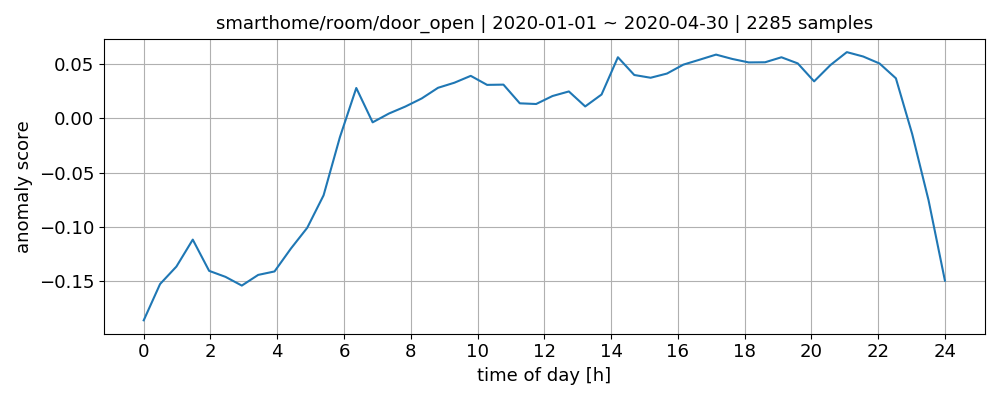
\includegraphics[width=0.95 \textwidth]{/plots/door_open.png}
  \caption{Graf popisující získané skóre pomocí klasifikace z natrénovaného modelu pro status dveří}
  \label{fig:app_door_open}
\end{figure}

Na \cref{fig:app_door_open} je zobrazen graf popisující pravděpodobnost změny statusu dveří. Model pro tuto veličinu byl natrénován na vzorcích z databáze v časovém rozmezí od 1. ledna 2020 do 30. dubna 2020 (za toto období bylo nasbíráno 2285 vzorků). \par
Na základě tohoto grafu můžeme popsat chování obyvatel domácnosti. V čase od přibližně 22 hodin do 6 hodin rána je velmi nepravděpodobné (skóre je záporné), že člen domácnosti otevře nebo zavře dveře. V průběhu dne je křivka v kladné části - v tuto dobu jsou dveře pravděpodobně často otevírány nebo zavírány. 

\subsubsection*{Pohyb v místnosti}

\begin{figure}[H]
  \centering
  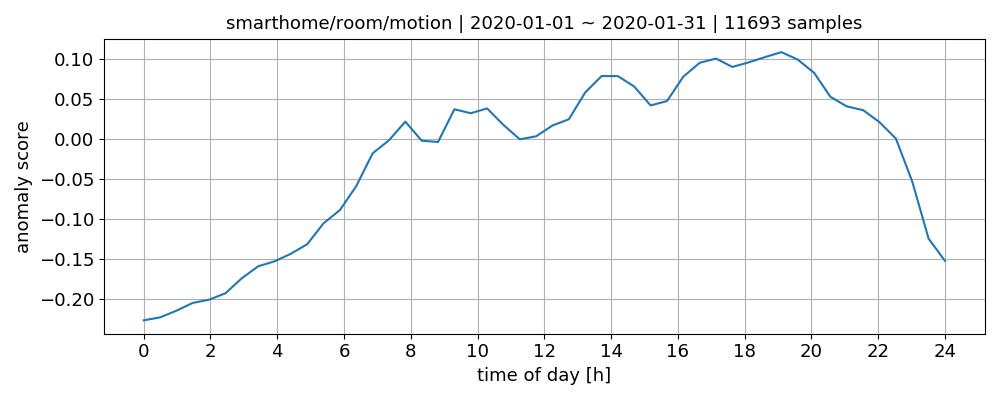
\includegraphics[width=0.95 \textwidth]{/plots/motion.png}
  \caption{Graf popisující získané skóre pomocí klasifikace z natrénovaného modelu pro pohyb v místnosti}
  \label{fig:app_motion}
\end{figure}

Na \cref{fig:app_motion} je graf zobrazující vývoj pohybu v místnosti v závislosti na časovém okamžiku. Model byl natrénován na vzorcích z časového období od 1. ledna 2020 do 31. ledna 2020 (11693 vzorků - tolikrát byl v místnosti zaznamenán pohyb). Analýza chování uživatele je podobná jako u předchozích jednodimenzionálních veličin - v noci uživatel spí a tudíž je pohyb v místnosti neočekávaný (záporné skóre). V průběhu dne se obyvatele domácnosti pohybují po místnosti a křivka je v kladné oblasti. 

\subsection*{Dvoudimenzionální veličiny}

\subsubsection*{Venkovní teplota}

\begin{figure}[H]
  \centering
  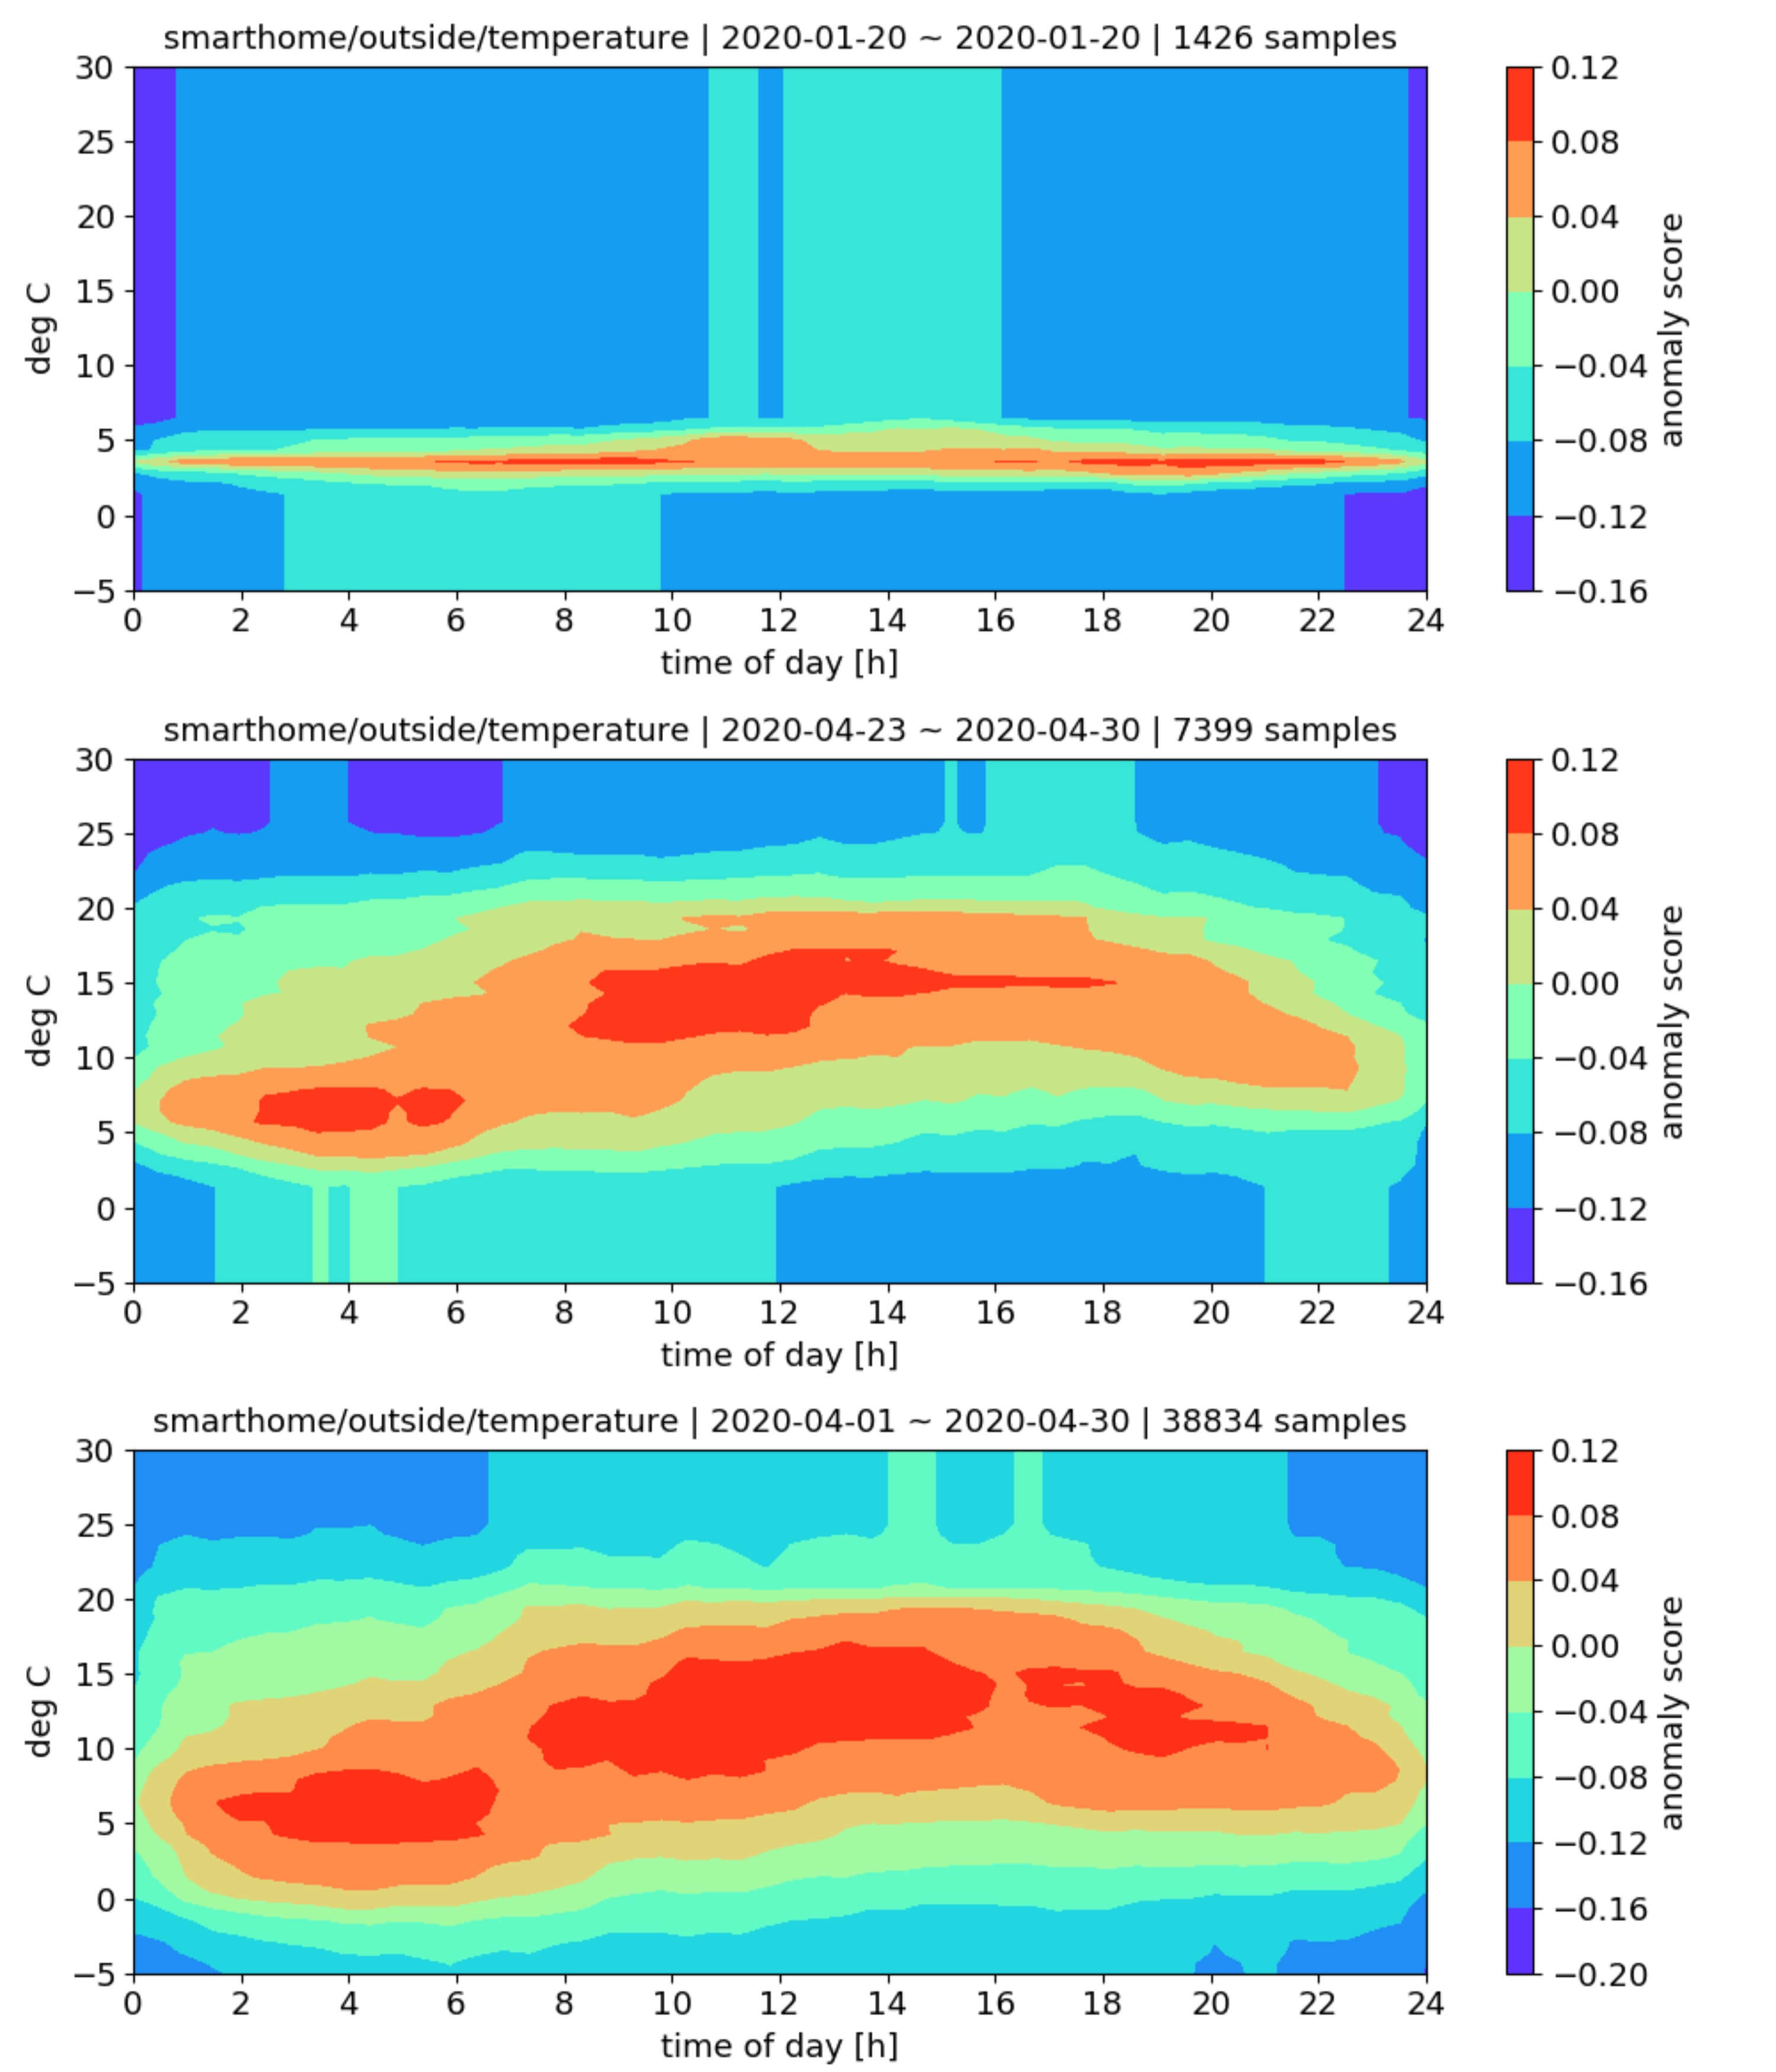
\includegraphics[width=0.95 \textwidth]{/plots/temperature_outside.jpg}
  \caption{Graf popisující získané skóre pomocí klasifikace z natrénovaného modelu pro venkovní teplotu}
  \label{fig:app_temperature_outside}
\end{figure}

Na \cref{fig:app_temperature_outside} jsou zobrazeny tři grafy ilustrující očekávaný vývoj venkovní teploty v průběhu dne na základě natrénovaných modelů pro různé časové období. První graf byl vygenerován pomocí klasifikace jednotlivých bodů na základě modelu natrénovaného ze vzorků za jeden den (20. ledna 2020). V tomto grafu lze vidět, že očekávaná venkovní teplota v průběhu celého dne byla okolo 4 \si{\degree}C. Prostřední graf byl získán klasifikací z modelu natrénovaného ze vzorků z databáze za období jednoho týdne od 23. dubna 2020 do 30. dubna 2020. Na rozdíl od prvního grafu lze vidět, že venkovní teploty pohybují ve větším rozmezí (dáno delším časovým rozmezím a jiným ročním obdobím) a očekává se, že budou dosahovat od přibližně 5 \si{\degree}C do 15  \si{\degree}C. Zajímavé jsou tmavě červené oblasti u přibližně 5  \si{\degree}C v čase od 2 do 6 hodin ráno a u 15  \si{\degree}C v čase od 9 do 15 hodin. Tyto oblasti byly ohodnoceny vysokým skóre - natrénovaný model očekává tyto hodnoty v tomto čase s velkou pravděpodobností. Na posledním grafu bylo rozšířeno časové rozmezí od 1. dubna do 30. dubna 2020 a model měl k dispozici 38834 vzorků v databázi. 

\subsubsection*{Vnitřní teplota}

\begin{figure}[H]
  \centering
  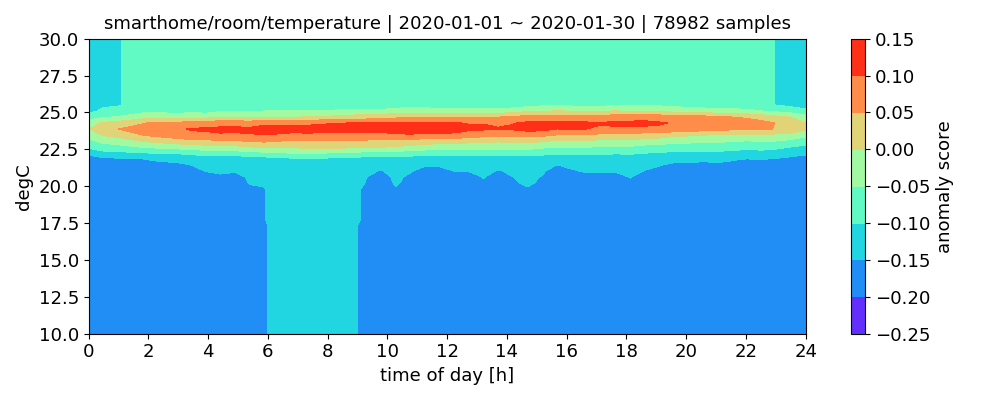
\includegraphics[width=0.95 \textwidth]{/plots/temperature_room.png}
  \caption{Graf popisující získané skóre pomocí klasifikace z natrénovaného modelu pro vnitřní teplotu}
  \label{fig:app_temperature_room}
\end{figure}

Na \cref{fig:app_temperature_room} je graf popisující očekávaný vývoj teploty v místnosti v průběhu dne na základě natrénovaného modelu pro tuto veličinu v časovém rozmezí od 1. ledna 2020 do 30. ledna 2020. Za toto období vzniklo 78982 vzorků (pozn.: vyšší počet vzorků u vnitřní teploty oproti venkovní teplotě za stejné období je dán vyšším počtem senzorů měřících vnitřní teplotu). Z tohoto grafu lze velmi přesně predikovat budoucí vývoj vnitřní teploty v místnosti - oblast, ve které model očekává hodnoty teploty je úzká od přibližně 22,5 \si{\degree}C do 25 \si{\degree}C. Rozsah vnitřní teploty je velmi omezený a v průběhu roku se téměř nemění. 

\subsubsection*{Barometrický tlak v místnosti}

\begin{figure}[H]
  \centering
  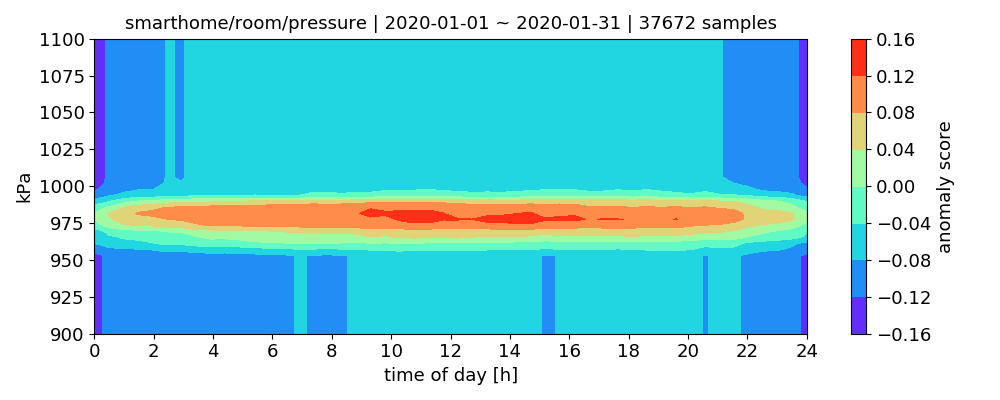
\includegraphics[width=0.95 \textwidth]{/plots/pressure_room.png}
  \caption{Graf popisující získané skóre pomocí klasifikace z natrénovaného modelu pro intenzitu osvětlení v místnosti}
  \label{fig:app_pressure_room}
\end{figure}

Na \cref{fig:app_pressure_room} je zobrazen graf ilustrující očekávaný vývoj barometrického tlaku v místnosti na základě klasifikace pomocí modelu natrénovaného pro tuto veličinu. Tento graf byl vygenerován pomocí modelu natrénovaného na přibližně 37 tisících vzorků v databázi. Hodnoty barometrického tlaku se stejně jako hodnoty vnitřní teploty pohybují v úzkém rozmezí a tyto hodnoty je možné velmi přesně predikovat. Za období měsíce ledna 2020 očekává natrénovaný model s největší pravděpodobností hodnoty okolo 975 kPa.

\subsubsection*{Vlhkost v místnosti}

\begin{figure}[H]
  \centering
  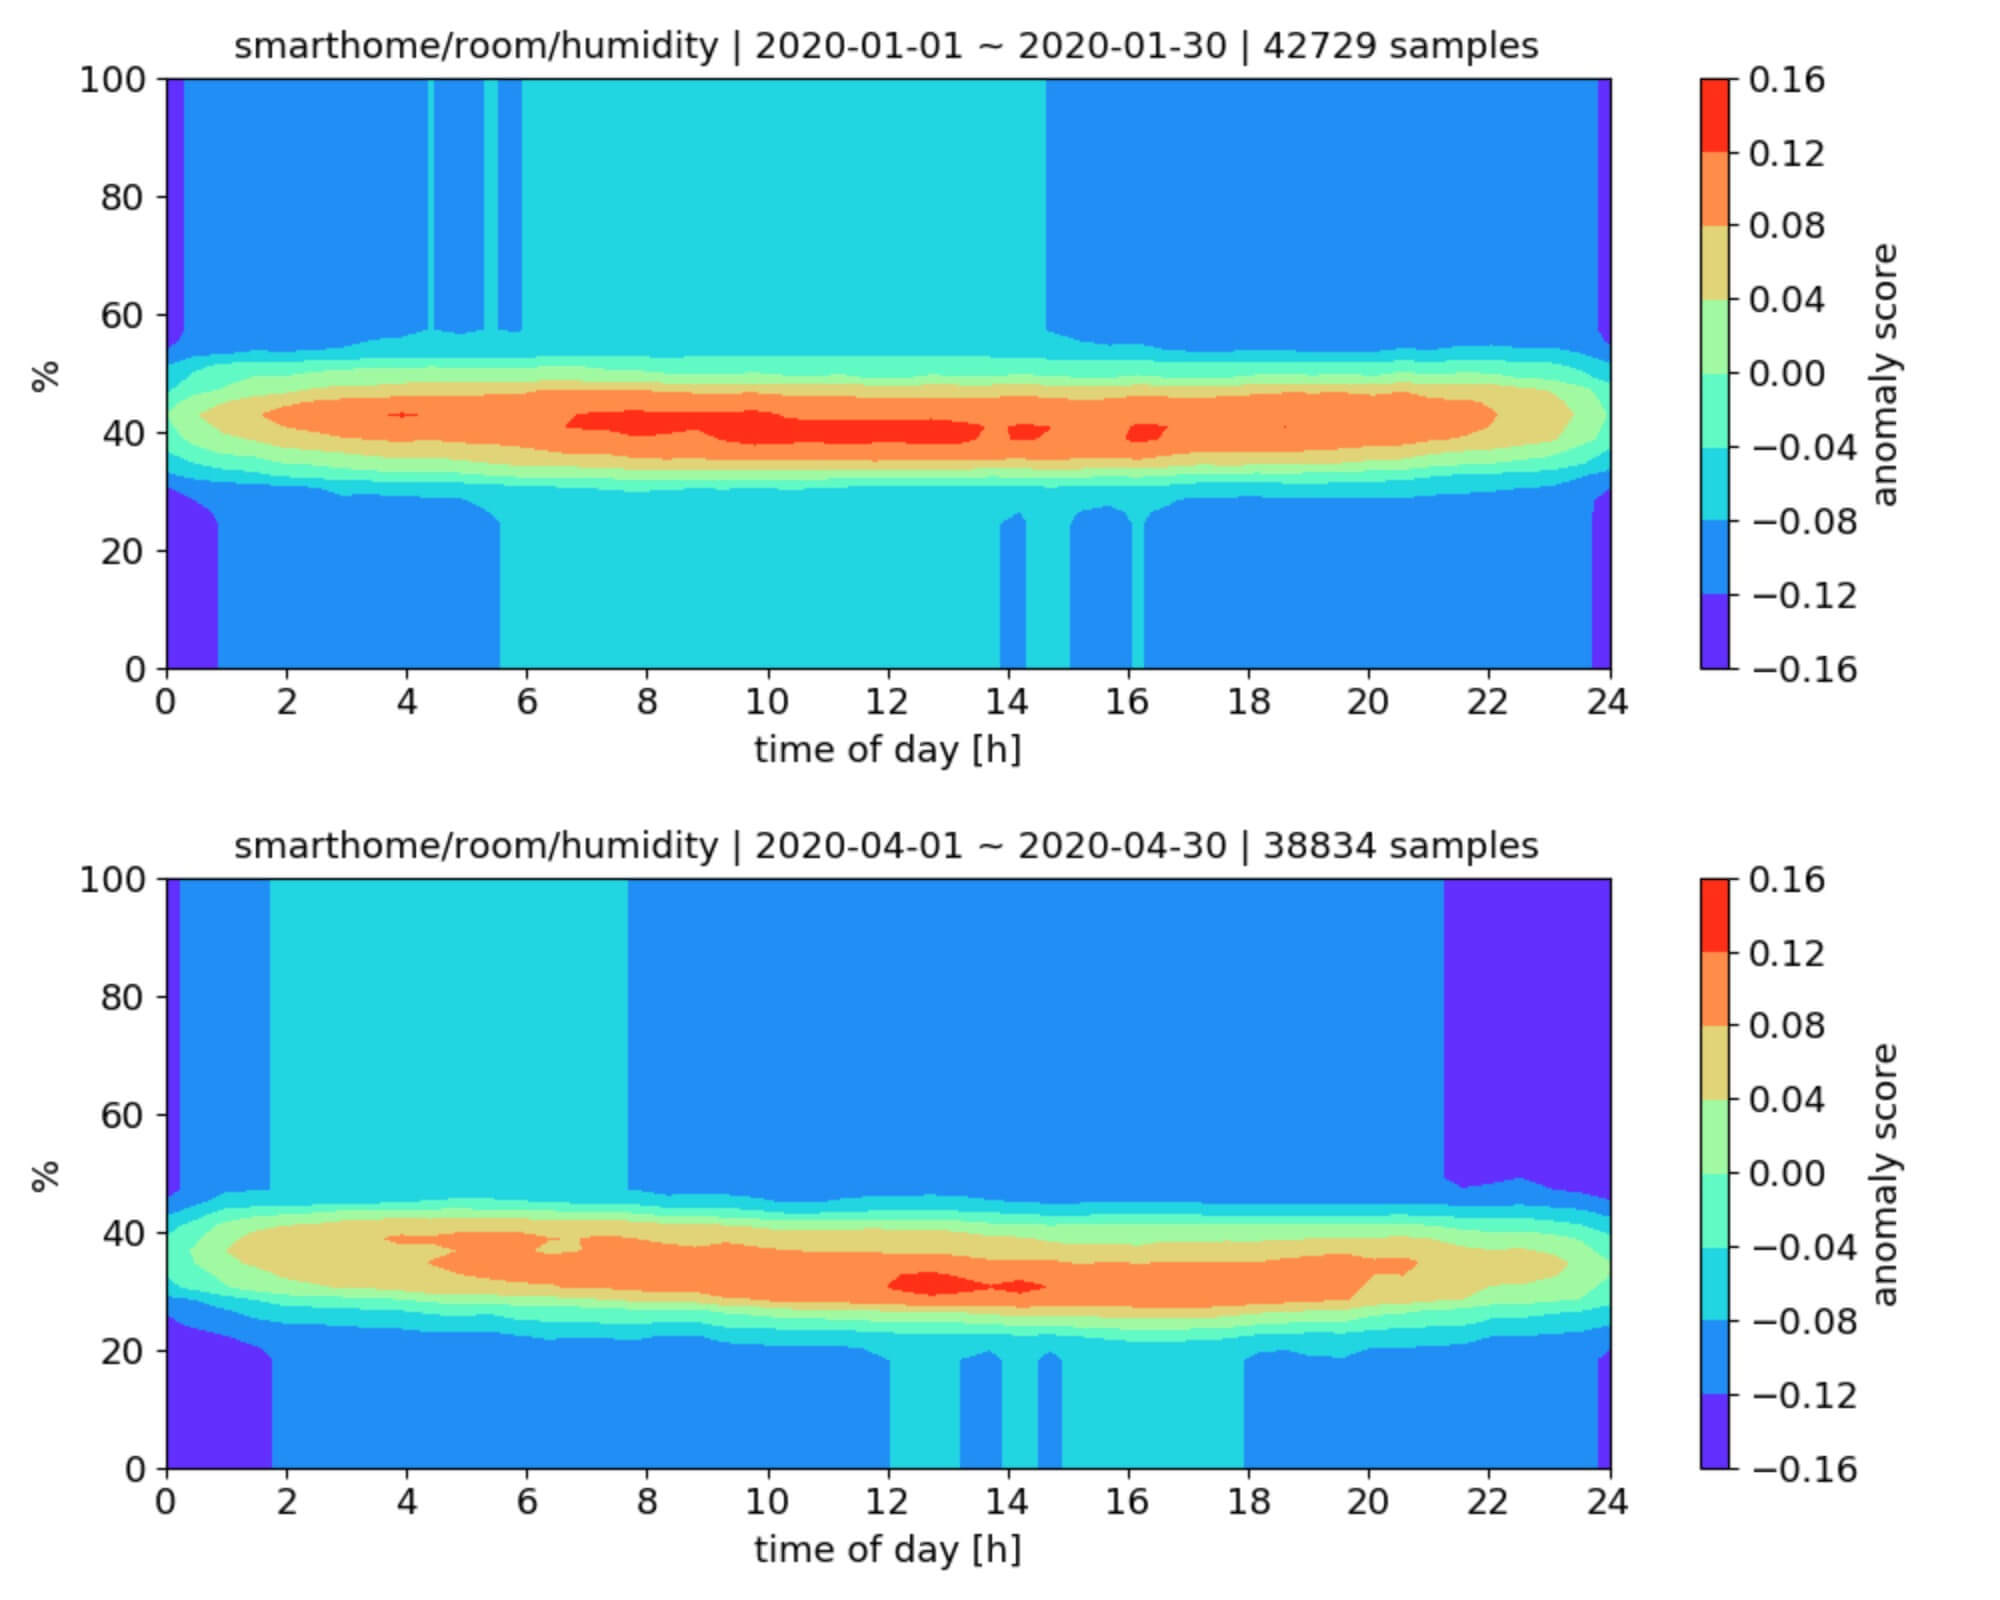
\includegraphics[width=0.95 \textwidth]{/plots/humidity_room.jpg}
  \caption{Graf popisující získané skóre pomocí klasifikace z natrénovaného modelu pro vlhkost v místnosti}
  \label{fig:app_humidity_room}
\end{figure}

Na \cref{fig:app_humidity_room} je zobrazen graf ilustrující očekávaný vývoj vlhkosti v místnosti na základě klasifikace jednotlivých bodů pomocí modelu natrénovaného ze vzorků z databáze. Horní graf byl vytvořen z přibližně 42 tisíc vzorků z časového období od 1. ledna do 30. ledna 2020, spodní graf ze vzorků za období od 1. dubna do 30. dubna 2020. Při porovnání obou grafů lze vidět, že hodnoty vlhkosti v místnosti nabývají úzkého rozsahu stejně jako u vnitřní teploty, ale tento rozsah hodnot se v průběhu roku posouvá. V grafu se vzorky za leden se vnitřní vlhkost pohybuje s největší pravděpodobností v rozmezí od 35 \% až 45 \% a v dubnovém grafu vnitřní vlhkost dosahuje nižších hodnot - od 25 \% do 35 \%. 


